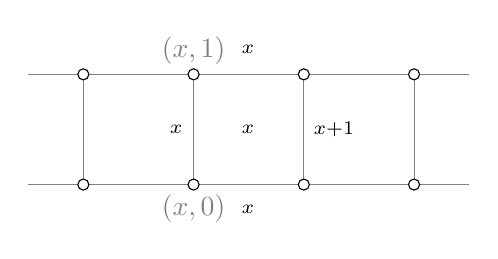
\begin{tikzpicture}[
        scale=0.7,
        site/.style = {circle, inner sep=0 pt, minimum size=4pt, draw=black, fill=white},
    ]
    \draw[step=2, Gray, thin] (-1,0) grid (7,2);

    \foreach \y in {0,2} \foreach \x in {0,2,...,6} \draw (\x,\y) node [site] {};

    \draw[Gray] (2,0) node [below] {$(x, 0)$};
    \draw[Gray] (2,2) node [above] {$(x, 1)$};

    \draw (2,1) node [left]  {$\runglink_x$};
    \draw (4,1) node [right]  {$\runglink_{x+1}$};
    \draw (3,0) node [below=4pt] {$\botlink_x$};
    \draw (3,2) node [above=4pt] {$\toplink_x$};
    \draw (3,1) node {$\square_x$};
\end{tikzpicture}
